\documentclass[10pt, pscyr, nonums]{hedlabwork}
\usepackage[russian]{babel}
\usepackage{hedmaths}
\usepackage{graphicx}
\graphicspath{{images/}, {plots/}}

\labnum{606}
\labname{Изучение работы счетчика Гейгера-Мюллера}
\student{Чечеткин И. А., Ф-469}
\date{30.10.2013}

\newgeometry{top=1.5cm, bottom=1.5cm, left=1cm, right=1cm}
\begin{document}
  \makeheader

  \emph{Цель работы:} ознакомление с аппаратурой и методикой, применяемой при
    регистрации заряженных частиц, изучение взаимодействия \( \alpha \),
    \( \beta \) и \( \gamma \) излучения с веществом.

  \begin{figure}[h!]
    \center
    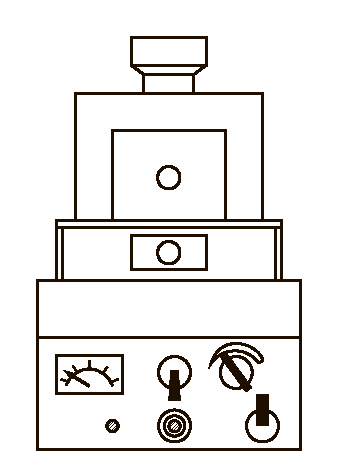
\includegraphics[width=.3\textwidth]{appearance}
    \caption{Внешний вид установки}
  \end{figure}

  \begin{table}[h!]
    \center
    \caption{Определение фона космического излучения}
    \begin{tabular}{|*{4}{C{.17}|}} \hline
      Время счета, мин &
        Количество зарегистрированных импульсов \( N \) &
        Фон \( n_\varphi \), имп/мин &
        Среднее значение фона \( \midnum{n}_\varphi \), имп/мин \\ \hline
      \multirow{3}{*}{3} & 36 & 12,0 & \multirow{3}{*}{11,7} \\ \cline{2-3}
      & 29 &  9,7 & \\ \cline{2-3}
      & 40 & 13,3 & \\ \hline
  \end{tabular}
  \end{table}
  
  \begin{table}[h!]
    \center
    \caption{Определение счетной характеристики газоразрядного счетчика}
    \begin{tabular}{|C{.15}|*{4}{C{.1}|}} \hline
      Напряжение на счетчике \( V \),~В &
        \multicolumn{3}{C{.3}|}{Количество импульсов, зарегистрированных
        за 1~мин \( n_0' \)} & \( \midnum{n_0'} \) \\ \hline
      260 &    0 &    0 &    0 &      0 \\ \hline
      280 &    0 &    0 &    0 &      0 \\ \hline
      300 &    0 &    0 &    0 &      0 \\ \hline
      320 &    0 &    0 &    0 &      0 \\ \hline
      340 & 1355 & 1380 & 1371 & 1368,6 \\ \hline
      360 & 1388 & 1412 & 1376 & 1392,0 \\ \hline
      380 & 1436 & 1385 & 1385 & 1402,0 \\ \hline
      400 & 1389 & 1370 & 1403 & 1387,3 \\ \hline
    \end{tabular}
  \end{table}

  \pagebreak
  
  \begin{table}[h!]
    \center
    \caption{Определение коэффициента поглощения алюминия}
    \begin{tabular}{|*{6}{C{.13}|}} \hline
      Толщина поглотителя,~м &
        Количество импульсов, \( N_1 \) &
        Интервал счета, мин &
        Скорость счета \( n_1 \),~имп/мин &
        \( \dfrac{n_0}{n_1} \) &
        \( \ln\dfrac{n_0}{n_1} \) \\ \hline
      \( 15 \cdot 10^{-5} \) & 1282 & \multirow{6}{*}{1} &
        1270,3 & 1,10 & 0,09 \\ \cline{1-2}\cline{4-6}
      \( 19 \cdot 10^{-5} \) & 913 &&
        901,3  & 1,54 & 0,43 \\ \cline{1-2}\cline{4-6}
      \( 26 \cdot 10^{-5} \) & 709 &&
        697,3  & 2,00 & 0,69 \\ \cline{1-2}\cline{4-6}
      \( 37 \cdot 10^{-5} \) & 679 &&
        667,3  & 2,09 & 0,74 \\ \cline{1-2}\cline{4-6}
      \( 43 \cdot 10^{-5} \) & 632 &&
        620,3  & 2,24 & 0,81 \\ \cline{1-2}\cline{4-6}
      \( 50 \cdot 10^{-5} \) & 582 &&
        570,3  & 2,44 & 0,89 \\ \hline
    \end{tabular}
  \end{table}
\end{document}
